\subsection{Class imbalance}
\label{sec:class_imbalance}
% \begin{figure}
%     \centering
%     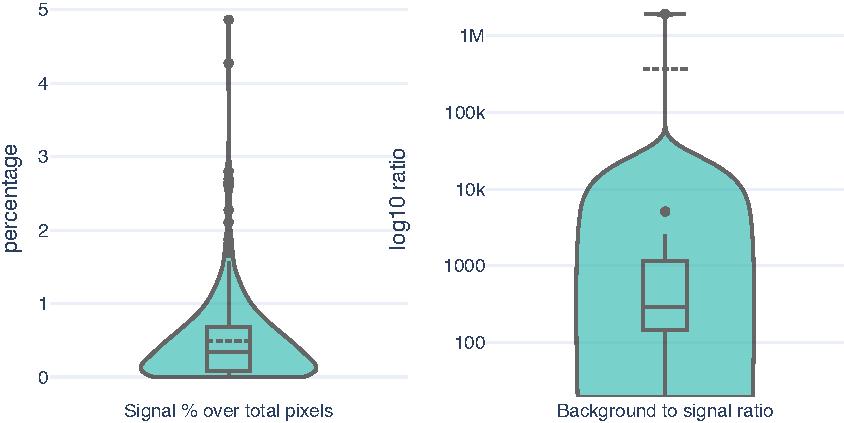
\includegraphics[width=\textwidth]{figures/120_dataset/features/class_imbalance.pdf}
%     \caption{\textbf{Class imbalance.} Violin plot and boxplot of signal percentage (left) and background to signal ration (right).}
%     \label{fig:dataset:class_imbalance}
% \end{figure}
\begin{figure}
    \centering
    \subfloat[Signal \% over total pixels]{
    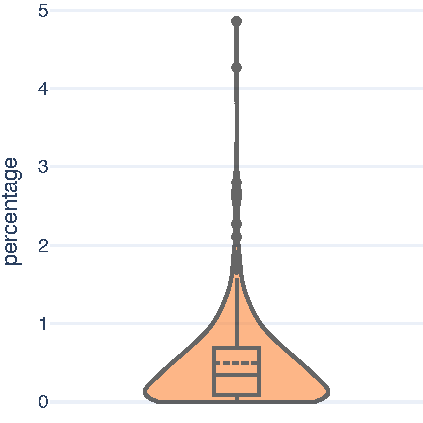
\includegraphics[width=0.5\textwidth]{figures/120_dataset/features/class_imbalance_percentage.pdf}\label{fig:dataset:class_imbalance:percentage}
    }
    \subfloat[Background to signal ratio]{
    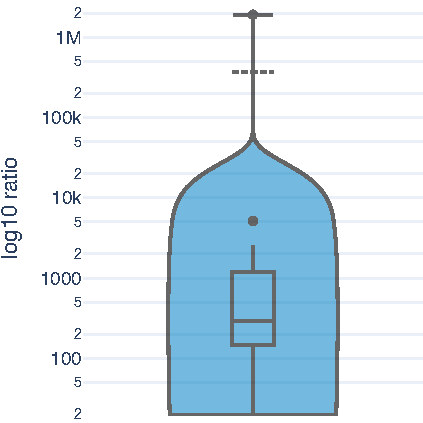
\includegraphics[width=0.5\textwidth]{figures/120_dataset/features/class_imbalance_ratio.pdf}\label{fig:dataset:class_imbalance:ratio}
    }
    \caption{\textbf{Class imbalance.} Violin plot and boxplot of signal percentage (\hyperref[fig:dataset:class_imbalance:percentage]{a}) and background to signal ration (\hyperref[fig:dataset:class_imbalance:ratio]{b}).}
    \label{fig:dataset:class_imbalance}
\end{figure}

Inspecting ground-truth masks at pixel level reveals important characteristics that affect the training process. 
By looking at the cardinality of pixels belonging to the background and the signal it is possible to notice how the two classes are extremely unbalanced (see \textit{signal (\%)}, and \textit{signal ratio} columns in \cref{tab:data_features} for a numeric summary).
\Cref{fig:dataset:class_imbalance:percentage} shows a violin plot of the percentage of signal pixel over the total image pixels across the 283 pictures.
The distribution is deeply skewed towards 0, with a median of 0.34\% and a 90\emph{-th} percentile of 1.07\%. 
Hence, almost 90\% of the images contain less than 1\% of pixels belonging to the signal%
% , causing an extreme unbalance between signal and background classes
.
Even more significantly, the right tail does not exceed 5\% of signal coverage, with a maximum of 4.86\%.

\Cref{fig:dataset:class_imbalance:ratio} illustrates the same concept but focuses on the relative proportion of background to signal. 
The distribution is left-skewed, with a lower half concentrated in the range (19, 291), i.e. background pixels are roughly from 20 to 300 times the signal pixels in 50\% of the images.
Remarkably, the disproportion grows even faster in the right tail, where the ratio explodes up to over 1000. 
Finally, notice that the bulk of outliers accumulates in the higher end of the domain. 
This is caused by the contribution of empty masks that cover more than 10\% of the total images.

These considerations expose the need for dedicated training strategies to face this strong class imbalance and correctly learn to classify image pixels.